\documentclass[a4paper,12pt,UTF8]{ctexart}
\usepackage{geometry}
\usepackage{cite}
\usepackage{indentfirst}
\usepackage{graphicx}
\usepackage{amsmath}
\usepackage{listings}
\geometry{a4paper,left=2.5cm,right=2cm,top=2.8cm,bottom=2.5cm}
\begin{document}
 毕设题目的内容主要有:\\
\indent 1.线控(主动)转向系统动力学建模\\
\indent 2.可变转向比的确定结合横摆角速度和质心侧偏角响应曲线(二自由度仿真建模)\\
\indent 3.转向电机的控制方法\\
\indent 4.程序流程图及程序的编写\\
\begin{figure}[htbp]
  \centering
  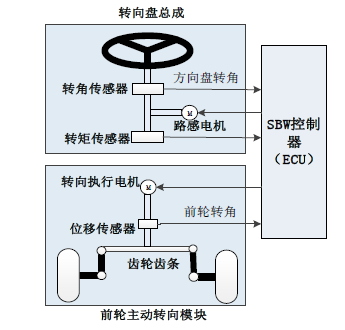
\includegraphics[width=10cm]{1.png}
  \caption{线控转向系统简图}
\end{figure}\\
\indent 如图1线控转向系统包括转向盘系统,车辆模型系统,前轮系统(包括电机和执行机构),控制器(ECU)。与传统转向系统不同,线控转向系统的转向盘系统与前轮系统之间通过电线连接,取消了传统的机械机构。取而代之的是一个控制器,控制器根据转向盘系统的输入信号来控制前轮系统。车辆模型系统本文采用二自由度车辆模型来计算。本文所做题目为主动转向模块程序设计,不包括路感设计,主要实现的是可变传动比和转向同步准确。电机控制考虑使用易于实现的PID增量式控制,跟随前轮转角,稳定性主要考虑横摆角速度和侧向加速度、质心侧偏角,稳定性可以和可变传动比中转向的灵敏度(横摆角速度增益)保持适宜相适应。\\
\begin{figure}[htbp]
  \centering
  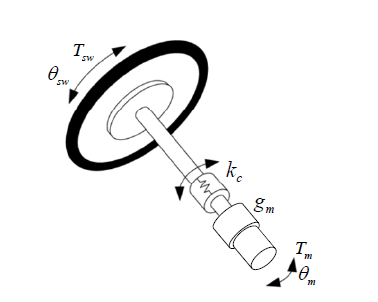
\includegraphics[width=10cm]{2.png}
  \caption{方向盘系统}
\end{figure}\\
 \indent如图2便是转向盘系统简图,包括转角传感器和力矩传感器以及路感电机。\\
 \indent 假设方向盘已经稳定即平衡,根据方向盘力矩平衡有:\\
\begin{equation}
  T_{sw}=J_{sw} \ddot{\theta}_{sw}+B_{sw} \dot{\theta}_{sw}+k_c(\theta_{sw}-\theta_m/g_m)+T_{fric}
\end{equation}
\indent 路感电机力矩平衡有:\\
\begin{equation}
  T_m=J_m \ddot{\theta}_m+B_m \dot{\theta}_m+\frac{k_c(\theta_m / g_m-\theta_{sw})}{g_m}
\end{equation}
\indent 路感电机电学平衡有:\\
\begin{align}
 T_m&=k_t I_a\\
 U_a&=R_a I_a+L_a \dot{I}_a+k_e \theta_m
\end{align}
\begin{figure}[htbp]
  \centering
  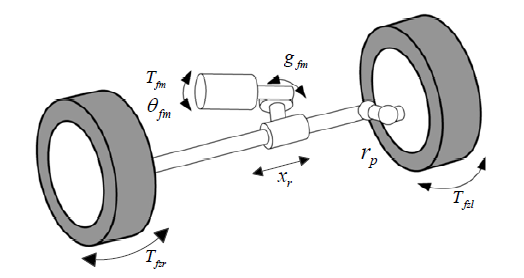
\includegraphics[width=10cm]{3.png}
  \caption{前轮系统}
\end{figure}\\
\indent 如图3便是前轮系统即转向执行机构主要包括转向器和转向电机,转向器采用的是齿轮齿条式。\\
\indent 同方向盘系统转向电机有以下平衡方程:\\
\begin{align}
  T_{fm} & =J_{fm}\ddot{\theta}_{fm}+B_{fm}\dot{\theta}_{fm}+\frac{k_{fc}(\theta_{fm}/g_{fm}-x_r/r_p)}{g_{fm}}\\
  T_{fm} & =k_{ft} I_{fa} \\
  U_{fa} & =R_{fa} I_{fa}+L_{fa} \dot{I}_{fa}+k_{fe} \theta _{fm}
\end{align}
\indent 转向器平衡有:\\
\begin{align}
  M_r \ddot{x}_r+B_r \dot{x}_r+F_{rack} &= \frac{k_{fc}(\theta _{fm}/g_{fm}-x_r/r_p)}{g_{fm}}) \\
  F_{rack} &= \frac{T_{fzl}}{l_{fl}}+\frac{T_{fzr}}{l_{fr}}
\end{align}\\
\indent 可变角传动比的确定\\
\indent 根据二自由度模型可得:
\begin{align}
  i&=\frac{u/L}{G^r_{\delta_{sw}}(1+Ku^2)}\\
  K&=\frac{m}{L^2}(a/k_2-b/k_1)
\end{align}
\indent 查资料得横摆角速度增益$G^r_{\delta_{sw}}$有以下关系\\
\begin{figure}[htbp]
  \centering
  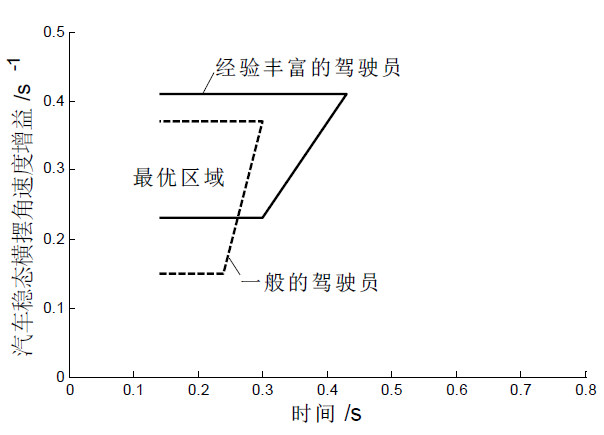
\includegraphics[width=10cm]{5.png}
  \caption{汽车理想稳态横摆角速度增益}
\end{figure}\\
\indent 取 $G^r_{\delta_{sw}}=0.319$得到角传动比与车速得关系如下图:\\
\begin{figure}[htbp]
  \centering
  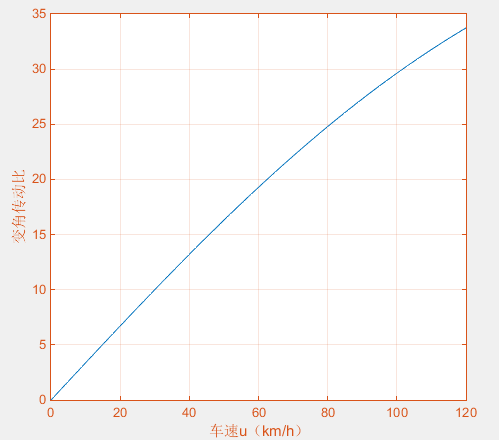
\includegraphics[width=10cm]{6.png}
  \caption{经验公式得到的角传动比与车速关系}
\end{figure}\\
\indent 考虑现实情况角传动比过大或过小都会影响汽车操作稳定性,故将上限定为$i_{max}=24$,下限为$i_{min}=10$。简单修正后如图:\\
\begin{figure}[htbp]
  \centering
  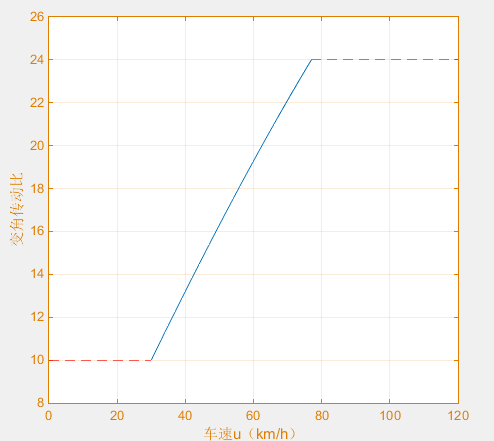
\includegraphics[width=10cm]{7.png}
  \caption{根据实际情况简单修正}
\end{figure}\newpage
\indent 函数式为:\\
\[i=f(u)=\begin{cases}
         i_{min} &  0 \leq x\leq30.00\\
         \frac{u/L}{G^r_{\delta_{sw}}(1+Ku^2)} &  30.00< x\leq76.97 \\
         i_{max} & u>76.97
       \end{cases}\]
\indent 考虑到曲线不连续,在拐点出现突变过程,影响驾驶员判断及其手感。现在利用matlab进行三次函数拟合。函数式为:\\
\[i=g(u)=\begin{cases}
         Au_3+i_{min} &  0 \leq x\leq u_0\\
         B(u-100)^3+i_{max} & u_0<x\leq 100 \\
         i_{max} & u> 100
       \end{cases}\]\\
\indent 拟合条件需要满足在拐点连续可导并且需要尽可能贴合原曲线,条件如下:\\
\begin{align*}
  g(u)_{u=u_0^-} & =g(u)_{u=u_0^+} \\
  \dot{g}(u)_{u=u_0^-}&=\dot{g}(u)_{u=u_0^+} \\
  max \xi=1-&\int_{0}^{120}[f(u)-g(u)]^2du
\end{align*}\\
\begin{figure}[htbp]
  \centering
  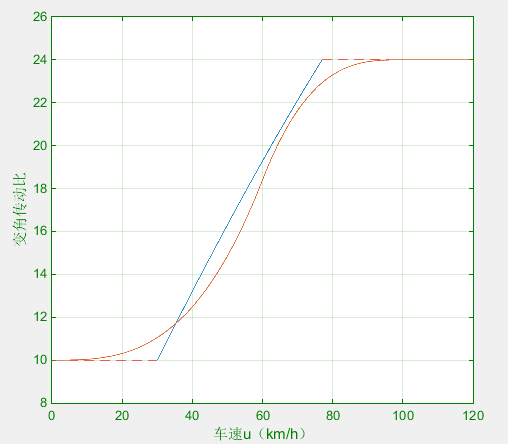
\includegraphics[width=10cm]{8.png}
  \caption{三次拟合修正}
\end{figure}\newpage
\indent 电机控制——增量式PID控制:\\
\begin{equation}
  \Delta u_k=k_p(e_k-e_{k-1})+k_i e_k+k_d(e_k-2e_{k-1}+e_{k-2})
\end{equation}
\begin{figure}[htbp]
  \centering
  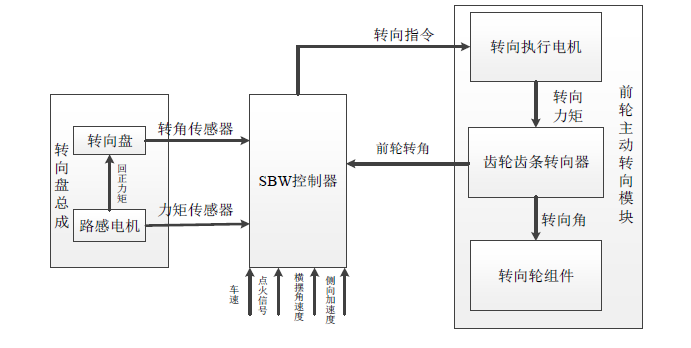
\includegraphics[width=10cm]{4.png}
  \caption{信号传递}
\end{figure}\\
\begin{figure}[htbp]
  \centering
  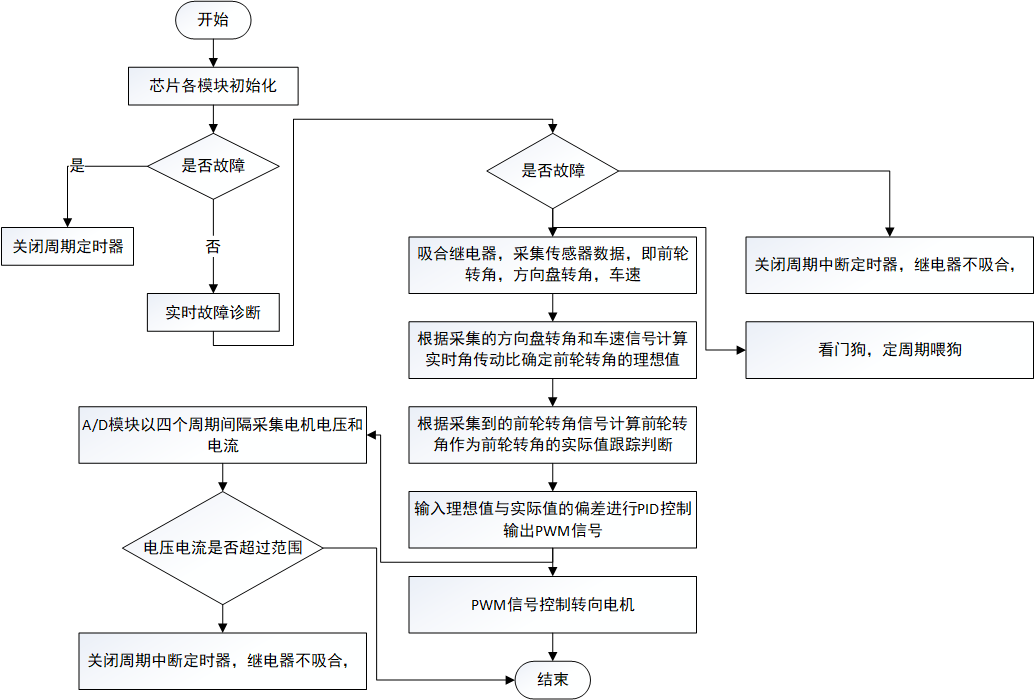
\includegraphics[width=16cm]{9.png}
  \caption{程序框图}
\end{figure}\\

\end{document}  